%!TEX root = ../tqft.tex

\begin{frame}[fragile]{Functorial field theories}
	\pause
	Monoidal functors from $\Bord_d$ to $\Vect_\CC$.

	\pause\medskip
	\colorit{Example:} For $d=2$, oriented theories are classified by commutative Frobenius algebras:
	\begin{center}
		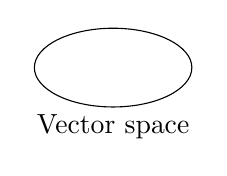
\begin{tikzpicture}[scale=.5]
			\draw (0,0) ellipse (2 and 1);
			\node[scale=1] at (0,-1.5) {\text{Vector space}};
		\end{tikzpicture}
		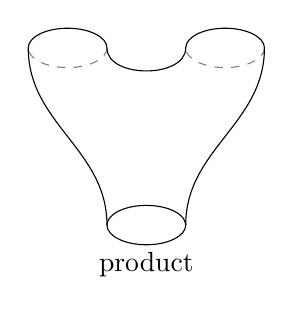
\begin{tikzpicture}[scale=.5]
			\draw (0,-.5) arc (0:-180: 1  and 0.5);
			\draw (0,-.5) arc (0:180: 1 and 0.5);
			\draw[dashed,color=gray] (-2,4) arc (0:-180: 1  and 0.5);
			\draw (-2,4) arc (0:180: 1 and 0.5);
			\draw[dashed,color=gray] (2,4) arc (0:-180: 1  and 0.5);
			\draw (2,4) arc (0:180: 1 and 0.5);

			\draw  (-2,-.5) to [out=90, in=-90] (-4,4);
			\draw  (0,-.5) to [out=90, in=-90] (2,4);
			\draw  (-2,4) to [out=-90, in=-90] (0,4);

			\node[scale=1] at (-1,-1.5) {\text{product}};
		\end{tikzpicture}
		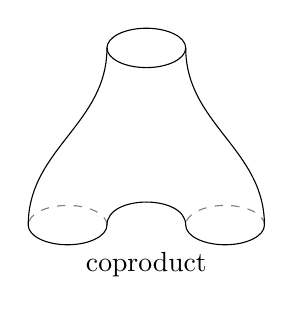
\begin{tikzpicture}[scale=.5]
			\draw (0,.5) arc (0:180: 1  and 0.5);
			\draw (0,.5) arc (0:-180: 1 and 0.5);
			\draw[dashed,color=gray] (-2,-4) arc (0:180: 1  and 0.5);
			\draw (-2,-4) arc (0:-180: 1 and 0.5);
			\draw[dashed,color=gray] (2,-4) arc (0:180: 1  and 0.5);
			\draw (2,-4) arc (0:-180: 1 and 0.5);

			\draw  (-2,.5) to [out=-90, in=90] (-4,-4);
			\draw  (0,.5) to [out=-90, in=90] (2,-4);
			\draw  (-2,-4) to [out=90, in=90] (0,-4);

			\node[scale=1] at (-1,-5) {\text{coproduct}};
		\end{tikzpicture}
	\end{center}

	\pause
	\colorit{Partition function:} To a closed top-dimensional manifold $M$ it assigns the number defining the morphism $\CC \to \CC$ defined by $M$.
\end{frame}

\begin{frame}[fragile]{State sum}
	\pause
	\colorit{Example:}
	Dijkgraaf--Witten invariant of a closed oriented 2-d manifold $M$.

	\pause\medskip
	Finite group $G$ with a $\rU(1)$-valued 2-cocycle $\omega$.

	\pause\smallskip
	States: $\set{\text{edges} \to G \mid \text{product of edges of a face is } 1}$

	\pause\medskip
	\colorit{Invariant:}
	\[
	Z(M) = \text{coeff} \
	\sum_{\substack{\text{states} \\ \phi}} \
	\prod_{\substack{\text{faces} \\ [012]}}
	\omega(\phi[01], \phi[12])^{\epsilon}
	\]
	where $\epsilon$ is $1$ or $-1$ based on the orientation.

	\pause\bigskip
	The group algebra $\CC[G]$ can be made into a Frobenius algebra using $\omega$ such that the associated field theory recovers $Z$ as its partition function.

	\pause\bigskip
	\colorit{Goal:} To keep the categorical nature \colorit{and} the local character of these two approaches.
\end{frame}

\begin{frame}{Street orientals}
	\pause
	The free $\omega$-categories generated by simplices.

	\begin{center}
		\includegraphics[scale=.25]{aux/street}
	\end{center}
\end{frame}

\begin{frame}{From simplicial sets to $\omega$-categories}
	\pause
	They form a cosimplicial $\omega$-category, and for any simplicial set $X$, let
	\[
	\cO(X) \defeq \colim_{\simplex^n \downarrow X} \cO_n
	\]

	\pause\bigskip
	The nerve of an $\omega$-category is defined, as usual, by the expression
	\[
	\rN(\cC)_k \defeq \omega\Cat(\cO_k, \cC).
	\]

	\pause\bigskip
	Analogous to the geometric realization and singular complex constructions.
\end{frame}

\begin{frame}[fragile]{State sum data}
	\pause
	Let $M$ be triangulated by $X$.
	To define a natural $\omega$-category morphism from $\cO(X)$ to some $\cC$, it suffices to define a cone under $\cO_\bullet$ with vertex $\cC$.
	\[
	\begin{tikzcd}
		\cO_0 \arrow[dr, bend right] \arrow[r,shift left=1] \arrow[r,shift right=1] &
		\cO_1 \dar \arrow[r,shift left=2] \arrow[r,shift right=2] \rar &
		\cO_2 \arrow[dl, bend left] \arrow[r,shift left=1] \arrow[r,shift right=1] \arrow[r,shift left=3] \arrow[r,shift right=3] & \cdots \\
		& \cC & \arrow[l,"\vdots"',pos=0.1, in=-20, out=200] &
	\end{tikzcd}
	\]

	\pause\medskip
	We refer to this as \colorit{state sum $\cC$-data}.

	\pause\medskip
	If $M$ is closed $n$-manifold and $\cC$ is sufficiently ``dualizable", the partition function of $M$  is the morphism in $\cC$ obtained by evaluating the fundamental cycle of $M$.

	\pause\medskip
	If $\cC$ is ``pointed" this morphism is identified with a complex number.

	\pause\medskip
	We will study the oriented case in more detail.
\end{frame}

\begin{frame}{Oriented case}
	\pause
	If we are interested in $n$-manifolds, we enhance the Street diagram with $n$-orientations by including both $\cO_n$ and $\cO_n^\op$.

	\begin{center}
		\includegraphics[scale=.05]{aux/two_triangles}
	\end{center}

	\pause
	If $M = \bars{X}$ is an oriented and triangulated manifold, we define $\cO_X(M)$ as before but $\cO_n$ or $\cO_n^\op$ depending if the canonical orientation of the simplex agrees with the induced from $M$.

	\begin{center}
		\includegraphics[scale=.05]{aux/composition}
	\end{center}
\end{frame}

\begin{frame}[fragile]{$B\Vect$}
	Let us consider the 2-category with one object, 1-morphisms given by $\Vect$ and composition by tensor product, and 2-morphisms given by linear maps.

	\pause\medskip
	A cone under
		\[
	\begin{tikzcd}[row sep=3]
		& & \cO_2 \\
		\cO_0 \arrow[r,shift left=1] \arrow[r,shift right=1] &
		\cO_1 \arrow[ru,shift left=2] \arrow[ru,shift right=2] \urar
		\arrow[rd,shift left=2] \arrow[rd,shift right=2] \drar & \\
		& & \cO_2^\op
	\end{tikzcd}
	\]
	with target $B\Vect$ is determined by a vector space $V$ with a product $\cdot$ and a coproduct $\Delta$.

	\pause\medskip
	\colorit{Question:} What about $\cO_3$?
\end{frame}

\begin{frame}{Relations}
	\pause
	Considering the multiple 2-oriented versions of $\cO_3$ we obtain a list of relations satisfied by $(V, \cdot, \Delta)$.
	\pause
	For example
	\begin{center}
		\includegraphics[scale=.06]{aux/frob_relation}
	\end{center}

	\pause
	\colorit{Observation 1.} These are satisfied if $(V, \cdot, \Delta)$ is a separable symmetric Frobenius algebra, which classify extended 2d-TQFT's.

	\pause\medskip
	\colorit{Observation 2.} These relations also imply the Pachner moves, so triangulation invariance.
\end{frame}

\begin{frame}{Towards the framed case}
	\pause
	There is a hierarchy of tangential structures to consider, the extreme cases are unoriented and framed.

	\pause\smallskip
	Let us consider a triangulated torus with the canonical framing
	\begin{center}
		\includegraphics[scale=.05]{aux/torus}
	\end{center}

	\pause\smallskip
	If in general position, the frame defines a 2-cat struct. on each simplex
	\begin{center}
		\includegraphics[scale=.03]{aux/framed_triangle}
	\end{center}
\end{frame}

\begin{frame}{Orientals after Kapranov Voevodsky}
	\pause
	Lets consider the convex closure of $n+1$ distinct points in the curve
	\begin{align*}
		\R &\to \R^{n} \\
		t &\mapsto (t,t^2,\dots,t^n)
	\end{align*}

	\pause
	The source and target of a $k$-face is obtained by projecting the last $n-k+1$ coordinates away and extremizing $e_k$ forward and backward
	\begin{center}
		\includegraphics[scale=.03]{aux/source_target}
	\end{center}

	\pause
	\colorit{Theorem(K-V).} These correspond to those constructed by Street.

	\pause\medskip
	\colorit{Question:} What about other frames?
\end{frame}

\begin{frame}[fragile]{Pasting schemes}
	\pause
	We quote Kapranov-Voevodsky:
	\begin{center}
		\includegraphics[scale=.23]{aux/kv}
	\end{center}

	\pause
	It cannot have loops
	\[
	\begin{tikzcd}
		\bullet \rar & \bullet \dar \\
		\bullet \uar & \bullet \lar
	\end{tikzcd}
	\]
\end{frame}

\begin{frame}[fragile]{Counterexample}
	\pause
	\colorit{Conjecture/claim (Kapranov-Voevodsky):} Any orthogonal frame in general position with respect to polytope $P$ defines via the previous construction a pasting scheme structure on it.

	\pause\bigskip
	\colorit{Construction (Laplante-M-Padrol)} An open family of frames in the $5$-simplex inducing a 2-loop.
	\[
	\begin{tikzpicture}[auto, node distance=2cm, >=latex',
		point/.style = {draw, circle, fill = black, inner sep = 1pt}]

		\coordinate (a) at (-3,-1);
		\coordinate (b) at (-2,1);
		\coordinate (c) at (-1,0);
		\coordinate (d) at (1,0);
		\coordinate (e) at (2,1);
		\coordinate (f) at (3,-1);

		\draw[thick] (c) -- (f) -- (b) -- (d);
		\draw[line width = 3pt,white] (d) -- (a) -- (e) -- (c);
		\draw[thick] (d) -- (a) -- (e) -- (c);
		\draw[thick] (a) -- (b) -- (c) -- (a);
		\draw[thick] (d) -- (e) -- (f) -- (d);

		\foreach \i in {a,b,...,f}
		{
			\node[point,label={above:$\i$}] at (\i) {};
		}

		\draw[->] (4,-1)-- (4,0);
		\draw[->] (4,-1)-- (5,-1);
		\node[] at (5.5, -1) {$e_1$};
		\node[] at (4.5, 0) {$e_2$};
	\end{tikzpicture}
	\]

	\pause
	\colorit{Construction (L-M-P)} A polytope where each frame induces a loop.
\end{frame}

\begin{frame}[fragile]{Toward the derived case}
	\pause
	My favorite definition of an $A_\infty$-algebra:

	\pause
	\[
	\begin{tikzcd}
		\cO_0 \arrow[dr, bend right] \arrow[r,shift left=1] \arrow[r,shift right=1] &
		\cO_1 \dar \arrow[r,shift left=2] \arrow[r,shift right=2] \rar &
		\cO_2 \arrow[dl, bend left] \arrow[r,shift left=1] \arrow[r,shift right=1] \arrow[r,shift left=3] \arrow[r,shift right=3] & \cdots \\
		& \rB\Ch & \arrow[l,"\vdots"',pos=0.1, in=-20, out=200] &
	\end{tikzcd}
	\]

	\pause\bigskip
	\colorit{Key idea:}
	\[
	\Omega^2 \cO_n \cong K_{n-2}.
	\]

	\pause\bigskip
	2-orientations give rise to a notion of ``Frobenius$_\infty$"-algebra.

\end{frame}

\begin{frame}{Conclusions and vague sentences}
	\begin{enumerate}
		\pause\item Functorial and state sum constructions of TQFT can be bridged using Street orientals. (State sum data is a cone over variations of Street's diagram.)
%		\pause\item This approach is conceptually novel and and explains combinatorially some of the structure that one finds in classification of TQFT.
		\pause\item The frame variation, which is initial among TQFTs, is related to the convex-geometric definition of $\omega$-cat structures on polytopes.
		(Kapranov--Voevodsky problem).
		\pause\item The conjectural answer of this problem is false.
		\pause\item Street orientals form a double desuspension of the Stasheff operad.
		Its 2-oriented version defines Calabi-Yau algebras.
		\pause\item (\colorit{Not} discussed today) Orientals and cup-$i$ products are combinatorially related, so one might hope for a connection between our functorial state sum viepoint and the classification of fermionic topological phases, done using cochains as fields with actions incorporating cup-$i$ products (Kapustin, Gaiotto, Thorngren, and others).
	\end{enumerate}
\end{frame}